\documentclass[12pt, a4paper]{report}
%\documentclass[11pt, a4paper]{article}

%====================== PACKAGES ======================
\usepackage[french]{babel}

\frenchbsetup{StandardLists=true}
\usepackage{enumitem}
\usepackage{pifont}

\usepackage[utf8x]{inputenc}
%\usepackage[latin1]{inputenc}

%pour gérer les positionnement d'images
\usepackage{float}
\usepackage{amsmath}
\usepackage{amssymb}
\usepackage{amsfonts}
\DeclareMathOperator{\dt}{dt}
\usepackage{graphicx}
%\usepackage{tabularx}
\usepackage[colorinlistoftodos]{todonotes}
\usepackage{url}

%pour les informations sur un document compilé en PDF et les liens externes / internes
\usepackage[pdfborder=0]{hyperref}
\hypersetup{
	colorlinks = true
	}

%pour la mise en page des tableaux
\usepackage{array}
\usepackage{tabularx}
\usepackage{multirow}
\usepackage{multicol}
\setlength{\columnsep}{50pt}

%pour utiliser \floatbarrier
%\usepackage{placeins}
%\usepackage{floatrow}

%espacement entre les lignes
\usepackage{setspace}

%modifier la mise en page de l'abstract
\usepackage{abstract}

%police et mise en page (marges) du document
\usepackage[T1]{fontenc}
\usepackage[top=2cm, bottom=2cm, left=2cm, right=2cm]{geometry}

%Pour les galerie d'images
\usepackage{subfig}

\usepackage{pdfpages}

\usepackage{tikz}
\usetikzlibrary{trees}
\usetikzlibrary{decorations.pathmorphing}
\usetikzlibrary{decorations.markings}
\usetikzlibrary{decorations.pathreplacing,calligraphy}
%\usetikzlibrary{decorations}
\usetikzlibrary{angles, quotes}
\usepackage{verbatim}

\usepackage{appendix}

\usepackage{comment}

\usepackage{xcolor}

%\PreviewEnvironment{tikzpicture}
%\setlength\PreviewBorder{0pt}%

%====================== INFORMATION ET REGLES ======================

%rajouter les numérotation pour les \paragraphe et \subparagraphe
\setcounter{secnumdepth}{4}
\setcounter{tocdepth}{4}

\hypersetup{							% Information sur le document
pdfauthor = {Stephan Runigo},			% Auteurs
pdftitle = {Documentation},			% Titre du document
pdfsubject = {Documentation},		% Sujet
pdfkeywords = {Document},	% Mots-clefs
pdfstartview={FitH}}	% ajuste la page à la largeur de l'écran
%pdfcreator = {MikTeX},% Logiciel qui a crée le document
%pdfproducer = {} % Société avec produit le logiciel

%======================== DEFINITION COMMANDES ========================
\newcommand{\fsb}[1]{\textsf{\textbf {\footnotesize #1}}}
\newcommand{\bi}[1]{\textbf{\textit {#1}}}
\newcommand{\si}[1]{\textsf{\textit {#1}}}
\newcommand{\lb}{$\lozenge$\ }
\newcommand{\bl}{$\blacklozenge$\ }
%======================== DEBUT DU DOCUMENT ========================
%
\begin{document}
%
% Titre, résumé, ... %
%
\begin{titlepage}
%
~\\[1cm]

\begin{center}
%\includegraphics[scale=0.5]{./presentation/chambreABulle}
\end{center}

\textsc{\Large }\\[0.5cm]

% Title \\[0.4cm]
\HRule

\begin{center}
{\huge \bfseries  La causalité\\
%titre 2\\[0.4cm]
 }
\end{center}

\HRule \\[1.5cm]

\begin{center}
%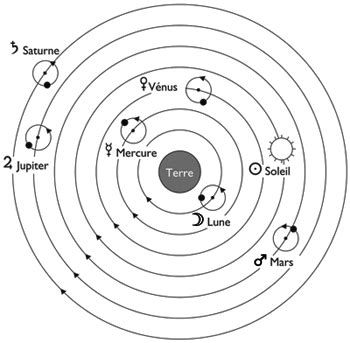
\includegraphics[scale=0.3]{./presentation/ptoleme}
\end{center}

\begin{center}
%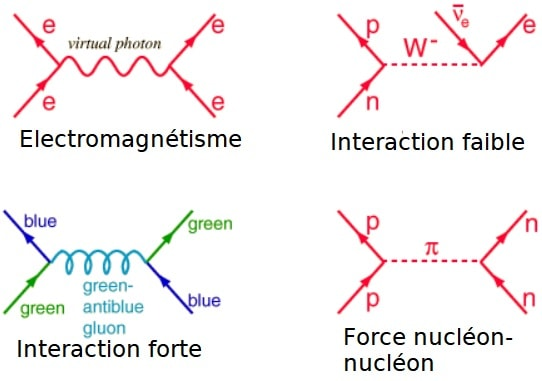
\includegraphics[scale=0.3]{./presentation/diagrammesInteractions}
\end{center}


% Author and supervisor
\begin{minipage}{0.4\textwidth}
\begin{flushleft} \large
%\emph{Auteur:}\\
%Stephan \textsc{Runigo}
\end{flushleft}
\end{minipage}
\begin{minipage}{0.4\textwidth}
\begin{flushright} \large
\emph{Auteur:}\\
Stephan \textsc{Runigo}
\end{flushright}
\end{minipage}

\vfill

% Bottom of the page
{\large \today}

\end{titlepage}

\newpage
\begin{center}
\Large
Résumé
\normalsize
\end{center}
\vspace{3cm}
\begin{itemize}[leftmargin=1cm, label=\ding{32}, itemsep=21pt]
\item {\bf Objet : } Souvenir des questions posés.
\item {\bf Contenu : } Définition, analyse, reflexion.
\item {\bf Public concerné : } Interressé à la question de l'âme.
\end{itemize}

\vspace{3cm}



\vspace{3cm}


%

% Table des matières
\tableofcontents
\thispagestyle{empty}
\setcounter{page}{0}
%
%====================== INCLUSION DES CHAPITRES ======================
%
~
\thispagestyle{empty}
%recommencer la numérotation des pages à "1"
\setcounter{page}{0}
\newpage
\chapter{Histoire}
%

\section{Vocabulaire}
\newpage
\subsection{cause}
	\begin{itemize}[leftmargin=1cm, label=\ding{32}, itemsep=11pt]

\ib{Causalité} — \si{Épist.} Rapport de cause*
à effet. — Principe de causalité :
« Tout a une cause et, dans les
mêmes conditions, la même cause
est suivie du même effet. »

\ib{Cause} — \si{Méta.} {\bf 1.} Force$^2$ productrice,
engendrant l'effet et se prolongeant
en lui. {\it cf.} {\it Efficace}* et {\it Occasionnelle}*. — \si{Épist.} {\bf 2.} Antécédent$^1$
constant (Hume) et inconditionnel
(J. S. Mill). — {\bf 3.} Phénomène lié au
phénomène considéré par une relation fonctionnelle : « La cause n’est
jamais vraiment empirique » (Bachelard) $->$ {\it Dans la science}, l'explication par les forces productrices
(sens 1) fait place de plus en plus à
l’explication par les relations fonctionnelles (sens 3). Aussi, tandis
que F. Bacon disait que « savoir
vraiment, c’est savoir par les causes »
(sens 2), A. Comte a pu écrire
(Cours, I) que la science renonce à
la recherche des causes (sens 1), ce
qui est d'ailleurs auj. discuté.

—— \si{Hist.} {\bf 4.} {\it Aristote} distingue
4 espèces de causes : a) la cause matérielle ({\it p. e.} dans une statue, la
matière dont elle est faite); — b) la
cause formelle (la figure que la statue
représente; {\it cf.} Formel); — c) la
cause efficiente, {\it i. e.} la cause au sens 1
(le sculpteur); — d) la cause finale$^1$
(le but : désir de la gloire ou du gain,
visé par le sculpteur).

— \si{Méta.} {\bf 5.} Cause première : voir
Premier$^4$.

	\end{itemize}
\subsection{effet}
	\begin{itemize}[leftmargin=1cm, label=\ding{32}, itemsep=11pt]

\ib{Effet} — \si{Épist.} {\bf 1.} Phénomène considéré comme produit par
une cause efficiente*. — \si{Psycho.} {\bf 2.} Loi de
l'{\it effet} : celle qui pose que « toutes
% 62
choses égales d’ailleurs, une réponse
est renforcée par le succès, affaiblie,
éliminée, ou remplacée à la suite de l'échec » (Lagache).

\ib{Efficace} — \si{Méta.} Qui produit réellement son effet : « Cause efficace »
({\it opp.} « occasionnelle* »).

\ib{Efficience} — \si{Épist.} {\bf 1.} ({\it Opp.} : {\it finalité}*).
Causalité efficiente* : « La
science ne peut s'intéresser à la finalité qu'après avoir épuisé tout son
effort dans la découverte de l’efficience » (F. Houssay).

— \si{Vulg.} {\bf 2.} [Angl. : {\it efficiency}].
Rendement, effet utile : « Le pragmatisme* est une théorie de
l’efficience de la connaissance. »

\ib{Efficiente (Cause)} — Celle qui « produit » l'effet (cf.
{\it efficace}*). Cette expression s'emploie  {\it auj.} comme
syn. de {\it cause}* tout court (aux
sens 1, 2 et même 3), et par {\it opp.}
à {\it cause finale} (cf. {\it Cause}$^4$). {\it Chez
Aristote}, au ctr., la cause efficiente
se subordonne à la cause finale :
c’est « l’activité qui sort du fond
même de l’être et tend à réaliser la fin » (Goblot).

	\end{itemize}

\subsection{hasard}
	\begin{itemize}[leftmargin=1cm, label=\ding{32}, itemsep=11pt]

\ib{Hasard} — \si{Vulg.} Ce qui n’est pas prévisible : {\bf 1.} soit qu’on
suppose dans les choses une indétermination$^2$ radicale ; — {\bf 2.} soit
qu'il s'agisse d'événements si complexes (cf. {\it Fortuit}*) qu’on ne puisse
en connaître toutes les conditions : « Il n’y a pas incompatibilité entre le
rôle de ce que nous appelons le hasard et l’établissement de lois
scientifiques » (Borel) ; — {\bf 3.} soit qu’on ignore le déterminisme$^1$ du
phénomène ; — {\bf 4.} soit que, se plaçant au point de vue de la finalité*,
on n’en aperçoive
% 86
pas les raisons d’être : « Ce qui est hasard à l’égard des hommes
est dessein à l'égard de Dieu » (Bossuet). $->$ Terme très équivoque.

	\end{itemize}

\newpage
\section{Solution ontologique et solution législative}

%https://www.sciencepresse.qc.ca/blogue/cerveau-niveaux/2019/05/14/faire-quand-survient-ecart-entre-theorie-observation
%https://fr.linkedin.com/pulse/r%C3%A9solution-ontologique-ou-l%C3%A9gislative-deli%C3%A8ge-builder-of-influencers
%https://forums.futura-sciences.com/archives/822692-solution-ontologique-legislative.html
%https://www.researchgate.net/publication/360773689_La_matiere_noire_une_enigme_de_la_cosmologie_contemporaine

L'observation du mouvement des planètes de notre système solaire s'est affinée au cours des temps. Les observations anciennes ont conduit à la mécanique aristotélicienne : les planètes ont un mouvement circulaire autour de la terre immobile. Des observations plus rigoureuse ont montré des mouvements plus compliqué que de simple cercle : cela à conduit à la théorie des épicycles.

Dix siècles plus tard, La révolution copernicienne conduit à l'invention de la mécanique newtonienne, qui s'impose face à la mécanique aristotélicienne.
%Face à des observations précises, une loi plus générale

La mécanique newtonienne permet de prédir les trajectoires des planètes de façon plus précise que la mécanique aristotélicienne.

Mais l'histoire ne s'arrète pas là. Des observations toujours plus précise vont conduire à découvrir que les trajectoires d'Uranus et de Mercure diffère des trajectoires calculées à partir de la nouvelle mécanique. Afin d'expliquer ces différences, des solutions vont finir par s'imposer.

Dans le cas d'Uranus, la solution va aboutir à la découverte d'une nouvelle planète : Neptune. Dans le cas de Mercure, la solution va aboutir à la découverte d'une nouvelle théorie : la relativité générale.

%La mécanique newtonienne permet de déduire la trajectoire des planètes de notre système solaire.

\newpage
\section{Le temps}

Les équations de newton font intervenir une variable. Newton appelera cette variable {\it temps}, concept existant se rapprochant le plus (pour Newton) de la variable introduite dans les équations.

\newpage
\section{Les quarks}

Les quarks sont les constituants des hadrons (proton, neutron, ...). Un neutron, comme un proton, est constitué de trois quark. Les quarks sont soumis à la force forte. Cette force, décrite dans la seconde moitié du {\footnotesize XX}$^\text{e}$ s., maintient les quarks entre eux.

Comme la force gravitationnelle maintient les planètes autour du soleil, la force électromagnétique maintient les électrons autour du noyau, la force forte maintient les quarks dans les protons et les neutrons. la force forte maintient également les protons et les neutrons dans les noyaux.

L'invention (la découverte) de la force forte a nécessité de baptiser de nouvelles grandeurs physiques.


\begin{center}
{\large\begin{tabular}{ccccc}
{\sf Interaction} & : & {\bf gravitationnelle} & {\bf électromagnétique} & {\bf forte} \\
{\sf remarque} & : & toujours attractive & attractive ou répulsive & toujours attractive ? \\
{\sf grandeur} & : & {\bf masse gravitationnelle} & {\bf charge électrique} & {\bf saveur} \\
{\sf remarque} & : & toujours positive & positive ou négative & 6 saveurs \\
\end{tabular}}
\end{center}


\newpage
\chapter{Formulaire}
\subsection{Mécanique analytique}

Action S et lagrangien L

Principe

\[
S = \int_{t_1}^{t_2} L(q_i, \dot{q}_i, t)dt \ \ \ \ \ \ \text{est extrémale}
\]

L'invariance du lagrangien par translation temporelle entraine le théorème :

\[
E \ \text{est une constante du mouvement}
\]

\subsection{Thermodynamique}

Énergie U, entropie S, température T, chaleur Q, travail W,  pression P, volume V

Principes
\[
dU = \delta Q + \delta W \ \ \ \ \ \ dS = \frac{\delta Q}{T}
\]
Théorème TdS
\[
dU = TdS - pdV
\]

\subsection{Quantique}
L'énergie est une observable, dans un système isolé,
\[
\mc{H}|\psi(x,t)\rangle=E|\psi(x,t)\rangle
\]


\[
\mc{H} = -i\hbar\frac{\partial}{\partial t} \ \ \ \ \ \ \ \mc{P} = i\hbar\frac{\partial}{\partial x}
\]

\newpage
\section{Onde et particule}
La physique classique (De Newton à Maxwell) distingue les phénomènes ondulatoires des phénomènes particulaires. Une onde se propage, s'étend, est susceptible d'interférence, une particule conserve sa forme, est susceptible d'en choquer une autre, suit une trajectoire.

\begin{center}
{\sf Figure : diffraction, interférence, choc, trajectoire.}
\end{center}

La nouvelle physique (quantique) unifie ces phénomènes, le nouveau paradigme ne distingue plus les ondes des particules, il n'y a que des quantons (ou des champs dans les théories les plus récentes $\to$ Feynmann).




\chapter{Dictionnaires}
\section{Larousse éthymologique}
{\bf énergie }{\footnotesize XV}$^\text{e}$ s. {\it Jardin de santé}, du bas latin {\it energia} (saint Jérôme), emprunté au grec {\it energeia}, force en action. || {\bf énergique} fin {\footnotesize XVI}$^\text{e}$ s. || {\bf énergétique} 1768, {\it Encycl.}, « qui paraît avoir une énergie innée »; sens actuel, fin {\footnotesize XIX}$^\text{e}$ s. (1909, L. M.); du grec {\it energetikos}.

{\bf Force} 1080, {\it Roland}, du bas latin {\it fortia}, pl. neutre subst. de {\it fortis}, courageux puis fort. || {\bf forcer} {\footnotesize XIII}$^\text{e}$ s. {\it Chr d'Antioche}, du lat. pop. {\it fortiare}, de {\it fortia}. [...]% || {\it forçage} {\footnotesize XII}$^\text{e}$ s.

\newpage
\section{Petit Larousse}

{\bf ÉNERGIE} {\sf n.f.} (gr {\it energeia}, force en action). {\bf I.1.} Force morale, fermeté, puissance, vigueur. {\it L'énergie du désespoir}. {\bf 2.} Vigueur dans la manière de s'exprimer. {\it Parler avec énergie}. {\bf 3.} Force physique, vitalité. {\it Un être plein d'énergie}. {\bf 4.} \fsb{PSYCHAN.} {\it Énergie psychique} ; libido. {\bf II.1.} \fsb{PHYS.} {\bf a.} Grandeur caractérisant un système et exprimant sa capacité à modifier l'état d'autres systèmes avec lesquels il entre en interaction (unité SI : le {\it joule}). {\bf b.} Chacun des modes que peut présenter un tel système. {\it Énergie mécanique, magnétique, nucléaire}. {\bf 2.} {\it Sources d'énergie} : ensemble des matières premières ou des phénomènes naturels utilisés pour la production d'énergie (charbon, hydrocarbures, uranium, cours d'eau, marées, vent, etc.).

$\blacksquare$ Outre l'énergie mécanique ({\it énergie potentielle} d'un poids soulevé, d'un ressort comprimé, etc., et {\it énergie cinétique} d'une masse en mouvement), on distingue les énergies {\it chimique, électrique, nucléaire, calorifique, rayonnante}. L'énergie est un concept de base de la physique car un système isolé a une énergie totale constante. Il ne peut donc y avoir création ou disparition d'énergie, mais seulement transformation d'une forme d'énergie en une autre ou transfert d'énergie d'un système à un autre. Toute conversion d'énergie s'accompagne de pertes. Celles-ci sont particulièrement importantes dans la conversion d'énergie thermique en énergie mécanique.

\vspace{0.24cm}
{\footnotesize 
{\bf ÉNERGÉTICIEN, ENNE} {\sf n.} Spécialiste d'énergétique.

{\bf 1. ÉNERGÉTIQUE} {\sf adj.} (angl. {\it energetic}). Relatif à l'énergie, aux sources d'énergie. \lb {\it Aliment énergétique :} aliment nécessaire à l'organisme pour réparer ses dépenses d'énergie et ses pertes de matière. {\bf —} {\it Apport énergétique :} apport d'énergie fourni à un organisme par un aliment, une boisson.

{\bf 2. ÉNERGÉTIQUE} {\sf n.f.} Science et technique de la production de l'énergie, de ses emplois et des conversions de ses différentes formes.

{\bf ÉNERGIQUE} {\sf adj.} {\bf 1.} Qui agit fortement ; efficace. {\it Un remède énergique}. {\bf 2.} Qui est plein d'énergie, qui manifeste de l'énergie. {\it Visage énergique}.

{\bf ÉNERGIQUEMENT} {\sf adv.} avec énergie.

{\bf ÉNERGISANT, E} {\sf adj. n.m.} Se dit d'un produit qui donne de l'énergie ; stimulant.

{\bf ÉNERGIVORE} {\sf adj. Fam.} Qui consomme beaucoup d'énergie.}
\vspace{0.31cm}

{\bf FORCE} {\sf n.f.} (bas lat. {\it fortia}, pl. neutre de {\it fortis}, courageux). {\bf I.1.} Énergie, vigueur physique. {\it Elle a beaucoup de force. \lb À force de :} à la longue, par des efforts répétés. {\it Force de la nature :} persone qui a beaucoup d'endurance, de résistance ou qui est pleine de vitalité. Tour de force : exercice corporel exigeant une grande force physique ; {\sf fig.}, résultat qui suppose une habileté, un effort exceptionnels. {\bf 2.} {\it Force de travail :} dans la terminologie marxiste, ensemble des facultés physiques et intellectuelles de l'homme, à l'aide desquelles il produit des choses utiles. {\bf 3.} Courage, capacité de résister aux épreuves. {\it Force d'âme, de caractère}. {\bf 4.} Degré d'aptitude dans le domaine intellectuel, niveau ; habileté. {\it Ils sont de la même force en maths}. {\bf 5.} Degré d'intensité (d'un sentiment). {\it La force du désir}. {\bf II.1.a} Emploi de moyen violents pour contraindre une ou plusieurs personnes. {\it Céder à la force. Employer la force. Coup de force.} \lb {\it De force, de vive force :} en employant la violence, la contrainte. {\bf —} {\it Par force :} sous l'effet de la contrainte. {\bf b.} {\it Épreuve de force :} situation résultant de l'echec des négociations entre deux groupes antagonistes et où la solution ne dépend plus que de la supériorité éventuelle de l'un sur l'autre. {\bf 2.a.} Ensemble de personnes armées et organisées, chargées d'une tâche de protection de défense ou d'attaque. \lb {\it Force publique :} ensemble des formations de la police, de la gendarmerie et des armées qui sont à la disposition du gouvernement pour assurer le respect de la loi et le maintien de l'ordre. {\bf b.} {\it Force de frappe, de dissuasion} ou, en France {\it force nucléaire stratégique :} force militaire aux ordres directs de la plus haute instance politique d'un État, rassemblant la totalité de ses armements nucléaires stratégiques. {\bf 3.} Pouvoir de ce qui incite ou oblige à se comporter d'une certaine manière. {\it La force de l'habitude} \lb {\it Par force :} par nécessité. {\bf —} {\it (Cas de) force majeure :} évènement imprévisible, contraignant ; nécessité qui impose à qqn sa conduite. {\bf 4.} Autorité, ascendant, pouvoir effectif. {\it La force des lois. Avoir force de loi.} {\bf —} \fsb{DR.} {\it Force exécutoire :} qualité d'un acte ou d'un jugement qui permet si besoin est, le recours à la force publique pour son exécution. {\bf III.} \fsb{PHYS}. Toute cause capable de déformer un corps, d'en modifier l'état de repos ou de mouvement. {\it Force d'inertie.} {\bf —} {\it Force électromotrice}, caractéristique d'une source d'énergie électrique qui crée un courant dans un circuit et détermine l'intensité de ce courant.{\bf —} {\it Force contre-électromotrice} $\to$ \bi{contre-électromotrice.} {\bf —} {\it Force d'un électrolyte :} mesure de son énergie de dissociation. {\bf IV.1.} Degré de puissance, d'intensité d'un agent physique. {\it La force d'un courant. Vent force 7.} {\bf 2.} Degré d'efficacité, de rendement de qqch. {\it La force d'un médicament. La force d'une machine.} {\bf V.1.} Importance numérique, quantité. \lb {\it Être en force :} être nombreux. {\bf 2.} {\it Faire force de rames, de voiles :} faire en sorte que les rames, les voiles déploient leur maximum de force. 
\bl {\sf pl.} {\bf 1.} {\it Forces (armées) :} ensemble des formations militaire d'un état. {\it Forces aériennes, navales, terrestre.} {\bf 2.} Ensemble des personnes unies par une même volonté, et œuvrant à sa réalisation. {\it Les forces de progrès.} 
$\blacksquare$ 
La notion de force tend à être remplacée par celle d'interaction. Un nombre restreint d'interactions fondamentales permet en effet de rendre compte de la complexité des phénomènes physiques. Outre l'interaction {\it gravitationnelle}, s'exerçant sur tous les systèmes possédant une masse, on distingue l'interaction {\it électrofaible}, rendant compte des phénomènes électromagnétiques et des phénomènes radioactifs, et l'interaction {\it forte}, responsable de la cohésion du noyau atomique.

\vspace{0.24cm}
{\footnotesize 
FORCÉ, E {\sf adj.} {\bf 1.a.} Qui manque de naturel. {\it Un rire forcé.} {\bf b.} Qui est imposé, que l'on fait contre sa volonté. {\it Atterrissage forcé.}{\bf —} {\it Avoir la main forcée :} agir malgré soi sous la pression d'autrui. {\bf 2.} {\it Marche forcée :} marche dont la durée et la rapidité dépassent celles des marches ordinaires. {\bf 3.} {\sf Fam.} Inévitable. {\it Elle gagnera, c'est forcé.} {\bf 4.} {\it Culture forcée :} culture de plantes soumises au forçage.
}
\vspace{0.31cm}

\newpage
\section{Petit Robert}

{\bf ÉNERGIE} {\sf n.f.} ( v. 1500 ; bas lat. {\it energia}, gr. {\it energeia} « force en action »).

{\bf I.} {\it cour.} \bl {\bf 1°} {\it Vieilli}. Pouvoir, efficacité (d'un agent quelconque). \lb Force , vigueur (dans l'expression, dans l'art). « {\it Quelle fraîcheur de coloris, quelle énergie d'expression} » ({\sc Rousseau}). « Une énergie singulière, un pittoresque effrayant » ({\sc Hugo}).
%
\bl {\bf 2°}(Fin {\footnotesize XVIII}$^\text{e}$). Force et fermeté dans l'action qui rend capable de grands effets. {\bf V. Dynamisme, ressort, volonté.} « {\it Cette énergie sublime qui fait faire les choses extraordinaires} » ({\sc Sthendal}). « {\it La quantité d'énergie ou de volonté que chacun de nous possède} » ({\sc Balzac}). « {\it Galvaniser nos énergie} » ({\sc Gide}). {\it Une énergie indomptable, farouche} « {\it L'internationale... avait perdu sa vitalité, tout en confisquant l'énergie du prolétariat} » ({\sc Romains}). {\it Regain d'énergie} {\bf V. Souffle} (second souffle). \lb Force, vitalité physique. {\it Se sentir plein d'énergie, frotter avec énergie.} « {\it Je le battis avec l'énergie obstinée des cuisiniers qui veulent attendrir un beafsteak} » ({\sc Baudelaire}).

{\bf II.} {\it Sc.} \bl {\bf 1°} {\it Phys.} (1875 ; angl. {\it energy}, 1852 ; sens plus vague 1807). Ce que possède un système s'il est capable de produire du travail. {\it Les différentes forme de l'énergie et leurs transformation. Énergie mécanique potentielle d'un corps} (Travail pouvant être produit en raison de la position d'un corps) ; {\it énergie cinétique} (acquise du fait de sa vitesse). {\it Énergie thermique} {\bf V. chaleur, thermodynamique.} {\it Énergie électrique, solaire} {\bf (V. rayonnement,)} chimique, nucléaire  {\bf (V. Radiation ; fission, fusion)}. {\it Principe de la conservation de l'énergie. Énergie interne,} en thermodynamique, somme des énergie potentielle et cinétique inhérentes à un système. {\it Les variations de l'énergie interne d'un système ne dépendent que de ses états initial et final.} \bl {\bf 2°} Énergie chimique potentielle de l'être vivant. {\it Énergie physiologique minimale} (ou métabolisme de base), dépense énergétique de l'organisme au repos complet.

$\boxdot$ {\sc Antonyme} \si{Indolence, inertie, mollesse, paresse.}

\vspace{0.24cm}
{\footnotesize 
{\bf ÉNERGÉTICIEN} {\it n. m.} (v. 1970 ; de énergétique). {\it Sc., techn.} Spécialiste de l'énergétique.

{\bf ÉNERGÉTIQUE} {\it adj.} et {\it n. f.} ( 1898 « qui parait avoir une énergie innée »; angl. energetic, gr {\it energêtikos}). \bl {\bf 1°} {\it Adj.} Relatif à l'énergie, aux grandeurs, aux unité, liées à l'énergie sous toute ses formes. {\it Puissance énergétique. Théorie énergétique}, système remplaçant en mécanique la notion de force par celle d'énergie. \lb Relatif à l'énergie utilisé industriellement. {\it Les ressources énergétique d'un pays.} \lb Physiol. {\it Dépense énergétique}, énergie qu'utilise l'organisme pour une action ou une fonction déterminée. {\it Aliments énergétiques}, qui fournissent beaucoup d'énergie à l'organisme. \bl {\bf 2°} {\it N. f.} Théorie énergétique. Science traitant des diverses manifestations de l'énergie.

{\bf ÉNERGIQUE} {\it adj.} (fin {\footnotesize XVI}$^\text{e}$; de {\it énergie}). \bl {\bf 1°} Actif, efficace. \bl {\it Un remède énergique.} {\bf —} Plein d'énergie (dans l'expression). {\bf V. Vigoureux.} \bl {\bf 2°}(fin {\footnotesize XVIII}$^\text{e}$). Qui a de l'énergie, de la volonté. {\bf V. Ferme, fort, mâle, résolu.} « {\it Un homme énergique n'a jamais peur en face du danger pressant} » ({\sc Maupassant}). {\bf —} qui exprime, marque de l'énergie. {\it Un visage énergique.} « {\it Une intervention énergique de la police} » ({\sc Martin du Gard}). \lb Fort, puissant (dans l'ordre physique). « {\it Un coup de pied... assez énergique pour briser les homoplates} » ({\sc Baudelaire}) $\boxdot$ {\sc ANTONYME} \si{Indolence, inertie, mollesse, paresse.}

{\bf ÉNERGIQUEMENT} {\it adv.} (1584; de énergique) Avec énergie. {\bf V. Fermement, résolument.} « {\it Fais énergiquement ta longue et lourde tâche} » ({\sc Vigny}). {\it Résister, protester énergiquement.} \lb Avec force « {\it Je serrai énergiquement cette main} » ({\sc Jaloux}).

{\bf ÉNERGISANT, E} {\it adj.} et {\it n.} (v. 1970 ; calque de l'angl. {\it energizing}). {\it Méd.} \bl {\bf 1°} {\it adj.} Qui stimule, donne de l'énergie. {\it L'action énergisante d'un médicament.} \bl {\bf 2°} {\it N. m.} Médicament qui stimule l'activité psychique. {\it Prendre des énergisant}. {\bf V. Antidépresseur, psychotonique, psychotrope.}
}
\vspace{0.31cm}

{\bf FORCE} {\sf n.f.} (1080 ;bas lat. {\it fortia}, plur. neutre substantivé de {\it fortis}. {\bf V. Fort ; forcer}).

{\bf I.} {\it La force de quelqu'un}. \bl {\bf 1°} Puissance d'action physique (d'un être, d'un organe). {\it Force physique ; force musculaire.} {\bf V. Résistance, robustesse, vigueur.} {\it La force du lion. Force de colosse, d'athlète. Avoir de la force.} {\bf V. fort.} {\it Ne plus avoir la force de marcher, de parler. Ne pas sentir sa force :} frapper, pousser, etc., trop fortsans s'en rendre compte. {\it Lutter à force égales, à égalité de forces.} « {\it Elle serrait la rampe avec tant de force que le bois grinçait} » ({\sc Green}). « {\it Patience et longueur de temps Font plus que force ni que rage} » ({\sc La Fontaine}) {\it Être à bout de force, sans force}. \lb {\it (Au plur.)} Ensemble, concours d'énergie. {\it Ménager ses forces. Ce travail est au-dessus de ses forces. Ses forces l'ont trahi. Reprendre des forces. Aliment qui redonne des forces :} fortifie, réconforte. {\it De toute ses forces :} en rassemblant et en utilisant toute ses forces ; {\it par ext.} le plus fort possible. {\it Il tapait, il criait de toutes ses forces.} \lb ({\it opposé} à adresse, souplesse) {\sc En force}, opposé à « en souplesse ». Courir, nager en force. {\bf —} {\sc De force} : qui exige de la force. {\it Tour de force. Épreuve de force. Travailleur de force :} personne dont le métier exige une grande dépense de force physique. {\it Travail, exercice de force.} \lb Mar. {\it Faire force} exercer ou imposer l'effort maximum. {\bf V. forcer.} {\it Faire force de rames :} ramer de toute ses forces. \lb Loc. {\it Dans la force de l'âge :} au moment ou un homme est le plus fort (maturité). \bl {\bf 2°} Capacité de l'esprit ; possibilités intellectuelles et morales. {\it La science des géomètres qui } « {\it exerce la force de l'esprit} » ({\sc Suarès}). « {\it Et consultez longtemps votre esprit et vos forces} » ({\sc Boileau}). Dans l'ordre moral. {\bf V. Constance, courage, cran, détermination, énergie, fermeté, volonté.} {\it Force morale ; force de caractère. La force d'âme des héros cornéliens.} « {\it Elle avait la force devant qui les autres plient : le calme} » ({\sc R. Rolland}). « {\it Elle me résistait avec une force de volonté qui voulait maîtriser la mienne} » ({\sc Loti}). {\it Ce sacrifice est au dessus de mes forces.} \bl {\bf 3°}  {\sc De} (telle ou telle) {\sc force.} {\it Ils sont de la même force} (physique morale). {\bf —} {\it Spécialement} (sur le plan intellectuel ou de l'habileté) {\it Ce joueur n'est pas de force. Ils sont de la même force au tennis, aux échecs, en mathématiques.} {\bf V. niveau.} \bl {\bf 4°} {\it Faire la force de qqn. :} constituer sa supériorité. « {\it Ce qui fait ma force c'est que je fais tout moi-même} » ({\sc Romains}).

{\bf II.} {\it La force d'un groupe, de qqch.} \bl {\bf 1°} Pouvoir, puissance. {\it La force de l'Église, d'un parti. Force militaire d'un pays.} Par ext. {\it La force publique :} les agents armés du gouvernement {\bf V. Police.} {\it La force armée :} les troupes. {\bf —} (1959) {\it Force de frappe :} ensemble des moyens militaires modernes (fusées, armes atomiques) destinés à écraser rapidement l'ennemi. Fig. (1961) Autorité, force, puissance. {\bf —} {\it Forces de dissuasion*. } {\bf —} {\sc prov.} {\it L'union fait la force.} \lb {\sc En force.} {\it Être en force ; arriver, attaquer en force :} en nombre, avec des effectifs considérables. \bl {\bf 2°} {\it Plur.} ({\footnotesize XVII}$^\text{e}$). Ensemble des armées. {\bf V. Armée, troupe}. {\it Les forces armées françaises. Forces navales, aériennes (1939). Forces terriennes} (F.T.A.). {\it Regrouper, concentrer ses forces. Les forces de police, les forces de l'ordre} (dans le langage gouvernemental, police et gendarmerie intervenant en cas d'émeutes). {\bf —} Par ext. {\it Forces politiques, syndicales.} « {\it Rallier les forces d'opposition} » ({\sc Martin du Gard}). \bl {\bf 3°} Résistance d'un objet. {\bf V. Résistance, robustesse, solidité.} {\it Force d'un mur, d'une barre.} Spécialt. {\it jambe de force}, ou {\it force :} pièce de charpente qui sert à soulager la portée des longues poutres. \bl {\bf 4°} Intensité ou pouvoir d'action d'une chose ; caractère de ce qui est fort (III). {\it La force du vent. Force d'un coup, d'un choc. Diminuer la force d'un son. La force d'un acide. Force d'un médicament.} {\bf V. Activité, efficacité.} \lb (Choses abstraites) {\it La force d'un sentiment, d'un désir :} son intensité.  {\bf V. violence.} « {\it un muscle perd sa vigueur, un désir sa force} » ({\sc Colette}). {\bf —} {\it Force d'un argument, d'une idée. Ici,} « {\it le mensonge a autant de force que la vérité} » ({\sc Green}). {\bf —} Loc. {\it Dans toute la force du mot, du terme :} dans l'acception la plus signifiante. {\bf —} {\it Force du style.} {\bf V. Couleur, vie vigueur.} {\it S'exprimer avec force.} {\bf V. Éloquence, feu, véhémence.} \bl {\bf 5°} Typogr. {\it Force de corps* d'un caractère :} mesuré en points. {\it Un corps de force 6} (du 6).

{\bf III.} ({\footnotesize XII}$^\text{e}$). Pouvoir de contrainte. \bl {\bf 1°} En parlant d'une personne, d'un groupe. {\bf V. Contrainte, oppression, violence.} {\it Employer alternativement la force et la douceur. Céder, obéir à la force.} {\bf —} {\it La force et la justice, et le droit. La force prime le droit}, mot attribué à Bismarck. {\it Le gouvernement menace de recourir à la force} (en employant des {\it forces} de police, la {\it force} publique ; Cf. {\it ci-dessus}, II). \lb {\sc De force}. {\it Coup de force.} {\bf —} Pouvoir de contraindre donné par la supériorité militaire. {\it Situation de force. Épreuve de force}, tout espoir de conciliation étant écarté. {\bf —} {\it Maison centrale de force :} prison d'État où sont les condamnés aux travaux forçés et à la réclusion. {\bf V. Forçat.} {\bf —} {\it Camisole de force.} \bl {\bf 2°} {\it La force de} (qqch.) : son caractère irrésistible. {\it La force de l'évidence :} devant laquelle on s'incline. {\it Faire qqch. par la force de l'habitude :} machinalement. {\bf —} {\it La force des choses} : la nécessité qui résulte d'une situation. {\bf V. Nécessité, obligation.} « {\it C'est précisément parceque la force des choses tend toujours à détruire l'égalité, que la force de la législation doit toujours tendre à la maintenir} » ({\sc Rousseau}). {\it Par la force des choses :} obligatoirement, inévitablement. {\bf —} {\it Force d'une loi}, son caractère obligatoire. {\bf V. Autorité.} {\it V. Autorité.} {\it Avoir force de loi :} être assimilable à une loi, en avoir le caractère obligatoire. \lb {\it Force majeure} (dr.) : évènement imprévisible, inévitable et irrésistible qui libère d'une obligation. Cour. C'est un cas de force majeur. \lb {\it Force est de... :} il faut, on ne peut éviter de... « {\it Force lui fût de reconnaître qu'... il avait opté pour le plus facile} » ({\sc Martin du Gard}). \bl {\bf 3°} {\it Loc. adv} {\sc De force} : en faisant effort pour surmonter une résistance. {\it Faire entrer de force une chose dans une autre. Prendre, enlever de force qqch. à qqn.} {\bf V. Arracher, extorquer} {\it Il obéira de gré ou de force :} qu'il le veuille ou non. {\bf —} {\it Loc. adv.} {\sc Par force} : en recourant à la force ; en cédant à la force. {\it Prendre, obtenir qqch. par force. Il n'a pas accepté de son plein gré, mais par force :} parce que les évènements l'y contraignaient. {\bf —} {\sc À toute force} : en dépit de tout les obstacles, de toute les résistances. {\bf V. absolument.} {\it Il voulait à toute force que nous l'accompagnions :} à tout prix, coûte que coûte.

{\bf IV.} Principe d'action physique ou morale. \bl {\bf 1°} Énergie, travail ({\it vx. en science}). \lb {\it Mod.} Toute cause capable de déformer un corps, ou d'en modifier le mouvement, la direction, la vitesse. {\it La mécanique, science de l'équilibre des forces et des mouvementqu'elles engendrent. Représentation vectorielle d'une force} (direction, sens, point d'application, intensité). {\it Résultante de deux forces. Équilibre des forces. Force d'inertie,} résistance qu'oppose une mobile à ce qui peut le mettre en mouvement. {\it Moment d'une force par rapport à un point. {\bf —} Spécialt.} Produit de la masse d'un corps par l'accélération que le corps subit (F $=$ m $\Gamma$). {\it Force vive d'un corps,} produit de la masse d'un corps par le carré de sa vitesse. {\it Force centrifuge, centripète. Force ascensionnelle d'un ballon. L'erg, unité de force dans le système C.G.S, le newton dans le système M.K.S.A. Force de contact} opposé à {\it forces de champ}, à distance. \lb {\it Lignes de force d'un champ électrique, magnétique.} Fig. {\it Les lignes de force d'une œuvre. {\bf —} Forces de gravitation, électromagnétiques, nucléaires. {\bf —} Force électromotrice*. {\bf —} (Électr.)} Courant électrique, et {\it spécialt.} courant électrique triphasé. {\it Faire installer la force chez soi.} \bl {\bf 2°} Principe d'action, cause quelconque de mouvement, dechangement. « {\it Notre volonté est une force qui commande à toutes les autres forces} » ({\sc Buffon.}) {\bf —} {\it Idées-force :} opinions ou idées capable d'influencer l'évolution d'un individu ou d'une nation, d'une époque. \lb {\it Les forces aveugles, mystérieuse, occultes de l'univers, du destin.} {\bf —} Fig. {\it C'est une force de la nature,} se dit d'une personne doué d'une vitalité irrésistible.

{\bf V.} {\sc À force.} {\it adv} (Vx). {\bf V. beaucoup, extrêmement.} « {\it Ne vois-tu pas le sang, lequel dégoutte à force...} » ({\sc Ronssard}). \lb Mod. {\sc À force de} {\it (Loc. prép.) :} par beaucoup de grâce à beaucoup de. {\it À force de patience, il finira par réussir.} {\bf V. Avec.} « {\it À force de plaisir, notre bonheur s'abîme} » ({\sc Cocteau}). {\bf —} Suivi d'un verbe, exprime la répétition, l'intensité. « {\it Quels cheveux sans couleur, à force d'être blonds !} » ({\sc Stendhal}). « {\it À force de penser à Marthe, j'y pensai de moins en moins} » ({\sc Radiguet}). {\bf —} {\it Ellipt.} {\sc À force.} {\it loc. adv.} (Fam.) À force, il a fini par y arriver.

$\boxdot$ {\sc Antonyme} \si{Affaiblissement, asthénie, débilité, faibless, fatigue. Apathie, inertie, molesse. Impuissance. Inefficacité. Douceur, persuasion.} {\bf —} {\sc Homonyme} \si{Forces.} Formes de forcer

2. {\bf Force} {\it adv.} (1337 ; du précéd.). {\it Vx} ou {\it littér.} Beaucoup. « {\it J'ai dévoré force moutons} » ({\sc La Fontaine}). « {\it Nous nou séparâmes à la porte avec force poignées de main} » ({\sc Daudet}). $\boxdot$ {\sc Homonyme} {\bf V. Force (1)}

{\bf FORCÉ, ÉE}. {\it adv.} ({\footnotesize XVI}$^\text{e}$, « involontaire ». {\bf V. Forcer}). \bl {\bf 1°} Qui est imposé par la force des hommes ou des choses. {\it Conséquence forcé}. {\bf V. Inéluctable, inévitable, nécessaire.} {\it Le mariage forçé}, comédie de Molière (1664). {\it Emprunt forçé}. {\bf V. obligatoire.} {\it Cours forçé d'une monnaie. Bagnard qui purge sa peine de travaux forçés} {\bf (V. forçat).} {\it L'avion a dû faire un atterrissage forçé. Un bain forçé.} {\bf V. involontaire.} {\it vente forçée. \lb Fam.} (Pour marquer le caractère nécessaire d'un évenement passé ou futur) {\it C'est forcé.} {\bf V. Évident, inévitable.} {\it Il perdra, c'est forcé !} {\bf V. forcément.} \bl {\bf 2°} {\it Vieilli.} Qui manque de sincérité ou de naturel. {\bf V. Affecté, artificiel, contraint, embarassé.} « {\it Vous vous moquez, me dit-il d'un air forcé} » ({\sc Marivaux}). Mod. {\it Un rire, un sourire forcé.} \bl {\bf 3°} Qui s'écarte du vrai ou du naturel. {\it Une comparaison forcée} (Cf. Tirée par les cheveux). {\it Effet forcé :} mal amené, trop recherché. $\boxdot$ {\sc ANTONYME} \si{Facultatif, libre, naturel, vrai.}


%
\begin{appendix}
%

%%%%%%%%%%%%%%%%%%%%%
\chapter{Glossaire}
%%%%%%%%%%%%%%%%%%%%%

\begin{itemize}[leftmargin=1cm, label=\ding{32}, itemsep=2pt]
\item {\bf application} : en mathématique, synonyme de fonction.
\item {\bf } :
\item {\bf } :
\item {\bf quanton} : particule élémentaire satisfaisant à l'équation de schrödinger.
\item {\bf } :
\item {\bf } :
\item {\bf } :
\end{itemize}


%%%%%%%%%%%%%%%%%%%%%%%%%%%%%%%%%%%%%%%%%%%%%%%%%%%%%%%%%%%%%%%%%%%%%%%%%%%%%%%%%%%%%

%

%%%%%%%%%%%%%%%%%%%%%
\chapter{Espace vectoriel}
%%%%%%%%%%%%%%%%%%%%%

%%%%%%%%%%%%%%%%%%%%%%%%%
\section{Ensemble et application}
%%%%%%%%%%%%%%%%%%%%%%%%%
%$\mathcal{}$
Un ensemble est une collection d'objets. Ces objets sont appelés éléments (a) de l'ensemble ($\mathcal{A}$) :
\[
 a \in \mathcal{A}
\]


Une application ($f$) met en relation chaque élément ($a$) d'un ensemble ($\mathcal{A}$, dit de départ) avec un élément ($b$) d'un autre ensemble ($\mathcal{B}$, dit d'arrivé) :
\begin{align*}
f :\ \ \ \ \ \ \ \ \ \mathcal{A} \ \  & \rightarrow \ \ \ \mathcal{B} \\
a \ \ & \mapsto \ \ b = f(a)
\end{align*}

Une loi de composition est une application qui associe deux éléments (éventuellement du même ensemble) à un troisième élément. 
\begin{align*}
f :\ \ \ \ \ \ \ \ \ \mathcal{A} \times \mathcal{B} \ \  & \rightarrow \ \ \ \mathcal{C} \\
(a,b) \ \ & \mapsto \ \ c = f(a,b)
\end{align*}

Une loi de composition est dite interne si $\mathcal{A} = \mathcal{B} = \mathcal{C}$, externe sinon.



%%%%%%%%%%%%%%%%%%%%%%%%%
\section{Espace vectoriel}
%%%%%%%%%%%%%%%%%%%%%%%%%
%
Un espace vectoriel est un ensemble (ses éléments sont appelés vecteur), possédant une loi de composition interne (la somme de deux vecteurs d'un espace vectoriel appartient à cet espace) et une loi de composition externe (la multiplication par un scalaire d'un vecteur d'un espace vectoriel appartient à cet espace).


%%%%%%%%%%%%%%%%%%%%%%%%%%%%%%%%%%%%%%%%%%%%%%%%%%%%%%%%%%%%%%%%%%%%%%%%%%%%%%%%%%%%%

%

%%%%%%%%%%%%%%%%%%%%%
\chapter{Transformation de fourier}
%%%%%%%%%%%%%%%%%%%%%

%%%%%%%%%%%%%%%%%%%%%%%%%
\section{Série de fourier}
%%%%%%%%%%%%%%%%%%%%%%%%%
%
Une fonction périodique (de période $T$) est égale à une somme discrète de sinusoïde :
\[
f_T(x)=a_0 + \sum_{n=1}^\infty \left( a_n \cos \frac{2 n \pi x}{T} + b_n \sin \frac{2 n \pi x}{T} \right)
\]
$a_n$ et $b_n$ sont les coefficient de fourier de $f_T(x)$.

%%%%%%%%%%%%%%%%%%%%%%%%%
\section{Transformé de fourier}
%%%%%%%%%%%%%%%%%%%%%%%%%
%
Une fonction quelconque est égale à une somme continue de sinusoïde :
\[
f(x) = \int_{-\infty}^\infty e^{2 i \pi \nu x}\widehat{f}(\nu) d\nu
\]
$\widehat{f}(\nu)$ est la transformé de fourier de $f(x)$.

%%%%%%%%%%%%%%%%%%%%%%%%%%%%%%%%%%%%%%%%%%%%%%%%%%%%%%%%%%%%%%%%%%%%%%%%%%%%%%%%%%%%%

%
%\newpage
%
\end{appendix}
%

%
%====================== INCLUSION DE LA BIBLIOGRAPHIE ======================
%
%récupérer les citation avec "/footnotemark" : 
\nocite{*}
%
% choix du style de la biblio
\bibliographystyle{plain}
%
% inclusion de la biblio
\cleardoublepage
\addcontentsline{toc}{chapter}{Bibliographie}
\bibliography{bibliographie.bib}
%
%====================== FIN DU DOCUMENT ======================
%
\end{document}
%%%%%%%%%%%%%%%%%%%%%%%%%%%%%%%%%%%%%%%%%%%%%%%%%%%%%%%%%%%%%%%%%%%%%%%%%%%%%%%%%
